\documentclass[conference]{IEEEtran}
\IEEEoverridecommandlockouts
% The preceding line is only needed to identify funding in the first footnote. If that is unneeded, please comment it out.
\usepackage{cite}
\usepackage{amsmath,amssymb,amsfonts}
\usepackage{algorithmic}
\usepackage{graphicx}
\usepackage{textcomp}
\usepackage{xcolor}
\usepackage[utf8]{inputenc} % allow utf-8 input
\usepackage[T1]{fontenc}    % use 8-bit T1 fonts
\def\BibTeX{{\rm B\kern-.05em{\sc i\kern-.025em b}\kern-.08em
    T\kern-.1667em\lower.7ex\hbox{E}\kern-.125emX}}
\usepackage{natbib}

\newcommand{\PeakNet}{PeakNet}
\newcommand{\peaknet}{PeakNet}
\newcommand{\psocake}{Psocake}

\begin{document}

\title{\peaknet{}: Bragg peak finding in X-ray crystallography experiments with
U-Net}

\author{\IEEEauthorblockN{Cong Wang}
\IEEEauthorblockA{\textit{Linac Coherent Light Source} \\
\textit{SLAC National Accelerator Laboratory}\\
%% 2575 Sand Hill Road, Menlo Park, CA 94025, USA \\
cwang31@slac.stanford.edu}
\and
\IEEEauthorblockN{Po-Nan Li}%*\thanks{* Performed this work in
%a previous role at SLAC National Accelerator Laboratory}}
%% City, Country \\
\IEEEauthorblockA{\textit{Department of Electrical Engineering} \\ 
\textit{Stanford University}\\
liponan@stanford.edu} %, Stanford, CA 94305, U.S.A
\and
\IEEEauthorblockN{Jana Thayer}
\IEEEauthorblockA{\textit{Linac Coherent Light Source} \\
\textit{SLAC National Accelerator Laboratory}\\
%% 2575 Sand Hill Road, Menlo Park, CA 94025, USA \\
jana@slac.stanford.edu}
\and
\IEEEauthorblockN{Chun Hong Yoon}
\IEEEauthorblockA{\textit{Linac Coherent Light Source} \\
\textit{SLAC National Accelerator Laboratory}\\
%% 2575 Sand Hill Road, Menlo Park, CA 94025, USA \\
yoon82@slac.stanford.edu}
}

\maketitle

\begin{abstract}
Serial crystallography at X-ray free electron laser (XFEL) sources has
experienced tremendous progress in achieving high data rate in recent times.
While this development offers potential to enable novel scientific
investigations, such as imaging molecular events at logarithmic timescales, it
also poses challenges in regards to real-time data analysis, which involves some
degree of data reduction to only save those features or images pertaining to the
science on disks.  If data reduction is not effective, it could directly result
in a substantial increase in facility budgetary requirements, or even hinder the
utilization of ultra-high repetition imaging techniques making data analysis
unwieldy.  Furthermore, an additional challenge involves providing real-time
feedback to users derived from real-time data analysis.  In the context of
serial crystallography, the initial and critical step in real-time data analysis
is finding X-ray Bragg peaks from diffraction images.  To tackle this challenge,
we present \peaknet{}, a Bragg peak finder that utilizes neural networks and
runs about four times faster than \psocake{} peak finder, while delivering
significantly better indexing rates and comparable number of indexed events.  We
formulated the task of peak finding into a semantic segmentation problem, which
is implemented as a classical U-Net architecture.  A key advantage of \peaknet{}
is its ability to scale linearly with respect to data volume, making it
well-suited for real-time serial crystallography data analysis at high data
rates.
\end{abstract}

%% \begin{IEEEkeywords}
%% component, formatting, style, styling, insert
%% \end{IEEEkeywords}

\section{Introduction}

Serial femtosecond crystallography (SFX) with X-ray free electron lasers (XFEL)
has enabled structural determination of macromolecules by outrunning radiation
damage at room temperature, an approach commonly known as
\textit{diffraction-before-destruction}
\citep{neutzePotentialBiomolecularImaging2000,
chapmanFemtosecondDiffractiveImaging2006,chapmanFemtosecondXrayProtein2011}.
Time-resolved serial femtosecond crystallography (TR-SFX) at XFEL facilities,
like the Linac Coherent Light Source (LCLS), allows the investigation of
biochemical reactions with picosecond time resolution which has led to many
significant structural studies
\citep{kupitzSerialTimeresolvedCrystallography2014,
nangoThreedimensionalMovieStructural2016,pandeFemtosecondStructuralDynamics2016a,
youngStructurePhotosystemII2016,sugaLightinducedStructuralChanges2017,
kernStructuresIntermediatesKok2018,ibrahimUntanglingSequenceEvents2020,
sugaTimeresolvedStudiesMetalloproteins2020} since the first published work at
LCLS \citep{aquilaTimeresolvedProteinNanocrystallography2012}.  In the meantime,
the data rate at XFEL facilities have also gradually increased from hundreds of
Hz to the MHz range, with the European X-ray Free Electron Laser (EuXFEL) being
the first MHz facility available to users and LCLS-II set to launch in 2023.

At the MHz data rate, novel real-time data analysis approaches are needed to
tackle two major challenges that arise in SFX experiments, namely data reduction
and real time feedback.  Firstly, data reduction aims to veto, extract and
compress scientific data by identifying important events, commonly referred to
as ``hits", and vetoing irrelevant ones from terabyte per second data streams.
One typical approach for SFX hit finding utilizes existing Bragg peak finders,
such as the Cheetah peak finder \citep{bartyCheetahSoftwareHighthroughput2014},
the robust peak finder \citep{hadian-jaziPeakfindingAlgorithmBased2017}, DIALS
peak finder \citep{Winter2018} or the \psocake{} peak finder
\citep{shinDataAnalysisUsing2018}.  Additionally, a neural network-based SFX hit
finder was reported to achieved a processing rate of 1.3 kHz on a single GPU
\citep{keConvolutionalNeuralNetworkbased2018}. ORB feature extractor combined
with a multilayer perceptron (MLP) hit classifier showed promising results for
SFX data \citep{rahmaniDataReductionXray2023}.  Secondly, real-time feedback in
SFX experiments provides users with information on the experimental conditions
and allows them to make real-time decisions that can optimize the data
acquisition process.  For example, it is critical to fine-tune the hit rate to
maximize the usage of collected data;  it is also important to know the current
diffraction limit, crystalline mosaicity, reciprocal space coverage, and other
relevant factors over time.  Therefore, hit finding alone is insufficient to
provide the necessary insights, making real-time Bragg peak finding crucial in
delivering fast and comprehensive feedback.  The previously mentioned peak
finder in \psocake{} runs at roughly 5 Hz on a data center CPU, which may result
in substantial cost when attempting to scale up the process.

In this work, we present \peaknet{} that addresses the problem of high data rate
peak finding by converting it into the task of peak segmentation using neural
networks.  To accomplish this goal, we propose to train a neural network model
to classify each individual pixel as either belonging to a peak or not belonging
to a peak.  This is followed by converting a connected area of pixels as a
single peak, a task that can be readily accomplished through connected component
analysis \citep{weaverCentrosymmetricCrossSymmetricMatrices1985}.  Subsequently,
the peak coordinates will be determined by computing the center of mass of all
the pixels that belong to the identified peak.  It is worth noting that the
entire peak finding process takes place on GPUs, offering a fully parallelizable
approach for achieving scalability.  Concretely, our contributions can be
summarized as follows:

\begin{itemize}

    \item We introduce a deep neural network-based Bragg peak finder, named
    \peaknet{}, which can effectively and efficiently segment hundreds or even
    thousands of Bragg peaks with various peak profiles in detector images of
    any dimension.  Despite being trained on peaks labeled by an existing peak
    finder, we highlight that \peaknet{}'s capability is not limited by the peak
    finder used in labeling.

    \item We demonstrate the efficacy of \peaknet{} by evaluating its
    performance on large multi-panel ($1739 \times 1748$) and single-panel
    ($1920 \times 1920$) detectors.  It significantly outperformed existing
    methods in terms of indexing rate, while delivering comparable number of
    indexed events.  We also fine-tuned the underlying U-Net architecture of
    \peaknet{} to strike an optimal balance between model efficacy and runtime
    performance, leading to a four times out-of-the-box processing speed
    improvement over \psocake{} peak finder.

\end{itemize}

%%%%%%%%%%%%%%%%%%%%%%%%%%%%%%%%%%% DIVIDER %%%%%%%%%%%%%%%%%%%%%%%%%%%%%%%%%%%

\section{Related work}

Reliable and automatic peak finding algorithms have undergone multiple
iterations of development.  An early approach involved utilizing template
matching \citep{wilkinsonIntegrationSinglecrystalReflections1988a} based on
libraries of peak shapes, but this method was found to be slow and inefficient
during runtime, especially when dealing with peaks with low signal-to-noise
ratios (SNR).  The main obstacle lies in the localization of peaks and the
tuning of user parameters for pattern matching, compounded by the difficult task
of developing a comprehensive library of peak shapes.  Another influential
approach employed region-growing techniques
\citep{bolotovskySeedSkewnessMethodIntegration1995,
bartyCheetahSoftwareHighthroughput2014} to detect pixel areas with high
skewness.  In the context of serial crystallography with XFEL sources, the
efficacy of this method was diminished due to the lack of sufficient data to
provide reliable statistics, rendering it susceptible to outliers and less adept
in analyzing weak peaks at higher scattering angles, which are essential for
achieving atomic resolution in structure determination.

While template matching and region-growing techniques require users to provide
prior information like threshold values, Robust Peak Finder (RPF)
\citep{hadian-jaziPeakfindingAlgorithmBased2017,
hadian-jaziDataReductionSerial2021} has demonstrated proficient peak finding
capabilities with minimal user input.  This technique utilizes the Modified
Selective Statistical Estimator (MSSE) method to segment between background
pixels and actual peaks.  Furthermore, the RPF method can also parallelize the
processing of diffraction patterns, making it suitable for real-time data
analysis.

\psocake{} is a software specifically designed to streamline high throughput
data reduction and analysis of XFEL experiments, and is routinely used at SLAC
National Accelerator Laboratory (SLAC) and Pohang Accelerator Laboratory (PAL).
The built-in peak-finding algorithm \citep{shinDataAnalysisUsing2018} includes
calibrating raw analog-to-digital units (ADUs); applying optional background
correction and bad pixel masks; identifying possible peaks; calculating their
SNR; determining Bragg spot sizes; and selecting peaks based on size, total
intensity and SNR.

In recent years, neural network models have emerged as a promising avenue for
Bragg peak finding.  BraggNet \citep{sullivanBraggNetIntegratingBragg2019} is
the first method that demonstrates proficiency of neural network models,
specifically U-Net \citep{ronnebergerUNetConvolutionalNetworks2015}, in
accurately segmenting peak pixels, including weak peaks, from background pixels
in neutron crystallography data.  Specifically, BraggNet employed simulated
peaks to create training datasets, which underwent a number of preprocessing
steps, including centering and cropping to a specific size and adding Poisson
noise.  It should be noted that BraggNet works on a single peak at a time within
a small 32 by 32 window, which deviates significantly from conventional Bragg
peak finding tasks that require extracting peak positions from images typically
with hundreds or thousands of pixels along one dimension.  Furthermore, another
neural network method for Bragg peak analysis was detailed in the work of
BraggNN \citep{liuBraggNNFastXray2021}, emphasizing the refinement of Bragg peak
positions without the need for explicit fitting of a profile function, such as
the pseudo-Voigt profile.  Likewise, BraggNN works on a single peak at a time
within a 11 by 11 window, performing regression to two variables representing
the peak position.  To the best of our knowledge, no existing neural network
based peak-finding models have demonstrated the ability to detect multiple peaks
with high precision without manual tuning of peak finding parameters, which is
the primary goal we strive to achieve with \peaknet{}.


%%%%%%%%%%%%%%%%%%%%%%%%%%%%%%%%%%% DIVIDER %%%%%%%%%%%%%%%%%%%%%%%%%%%%%%%%%%%

\section{Methods}

% Summarize the method
% Breakdown
% - u-net
% - loss function
% - post process
% - labeling
%   - stream files, peak found and indexed
%   - label refinement

\peaknet{} uses a U-Net architecture to perform peak segmentation on diffraction
images, generating a heatmap of probabilities of a given pixel belonging to a
true peak.  A probability threshold is subsequently employed to translate the
heatmap into a binary mask or segmentation map, with a value of one indicating a
peak pixel and zero otherwise.  A connected component analysis
\citep{weaverCentrosymmetricCrossSymmetricMatrices1985} is then applied to
extract peak positions in image coordinates.  The entire peak finding process is
summarized in Fig. \ref{fig : peak finding}.  In this section, we present the
details in model training, comprising the specific U-Net architecture, the loss
function and the data labeling process.

\begin{figure*}[htbp]
\centering
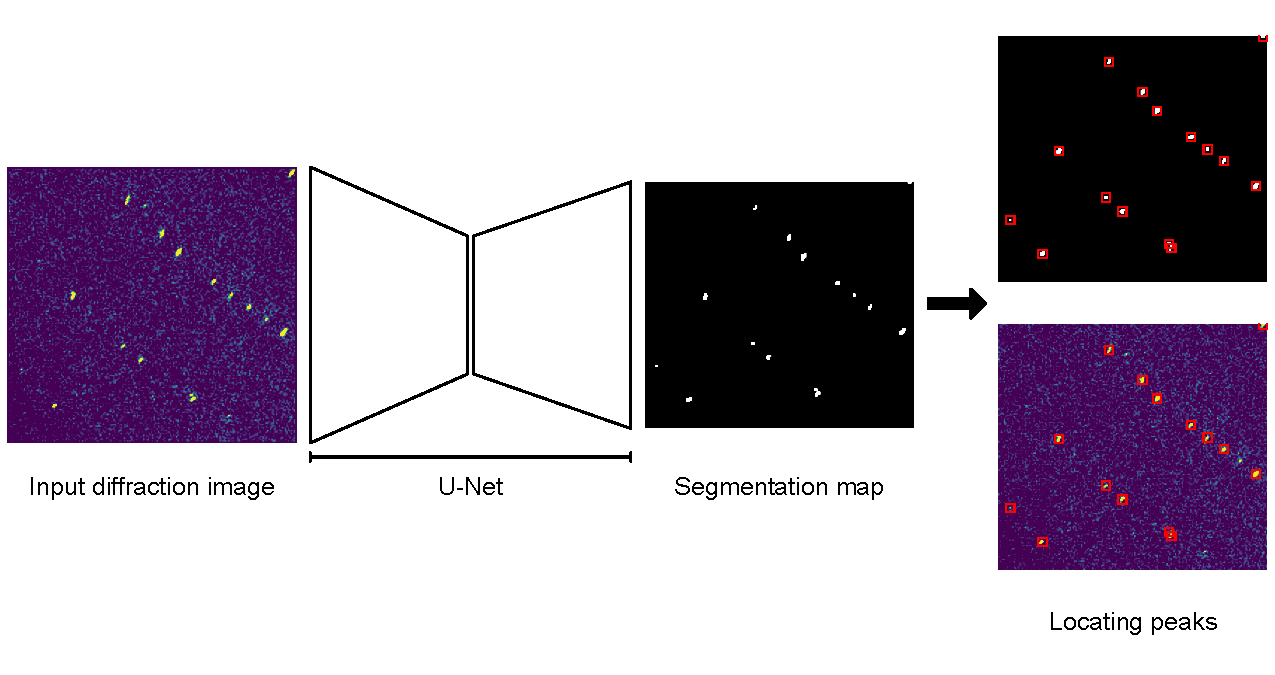
\includegraphics[width=0.9\textwidth,keepaspectratio]
{./figures/peaknet.method.pdf}
\caption{Peak finding process in \peaknet{}.}
\label{fig : peak finding}
\end{figure*}


\subsection{The segmentation model: U-Net}

Peak segmentation in \peaknet{} is achieved by the use of U-Net
\citep{ronnebergerUNetConvolutionalNetworks2015} with a reduced number of
feature channels applied in both the contracting and expanding paths, as
depicted in Fig. \ref{fig : unet}.  A single contracting layer contains two
stride-one and zero-padding $3 \times 3$ convolutional layers with a rectified
linear unit (ReLU) \citep{fukushimaCognitronSelforganizingMultilayered1975} and
an additional stride-two $2 \times 2$ max-pooling layer.  The number of feature
channels doubles with respect to its previous contracting layer.  Likewise, a
single expanding path contains a stride-two $2 \times 2$ transposed
convolutional layers concatenated with the corresponding feature map from the
contracting path.  This is followed by two stride-one $3 \times 3$ convolutional
layers connected to a ReLU activation function.  It is worth noting that the
feature map cropping may be necessary during the concatenation between feature
maps from two paths.  In the last layer, all 8 channels will be mapped to a
single channel through a $1 \times 1$ convolution.

\begin{figure*}[htbp]    % Insert the figure HERE and TOP
\centering
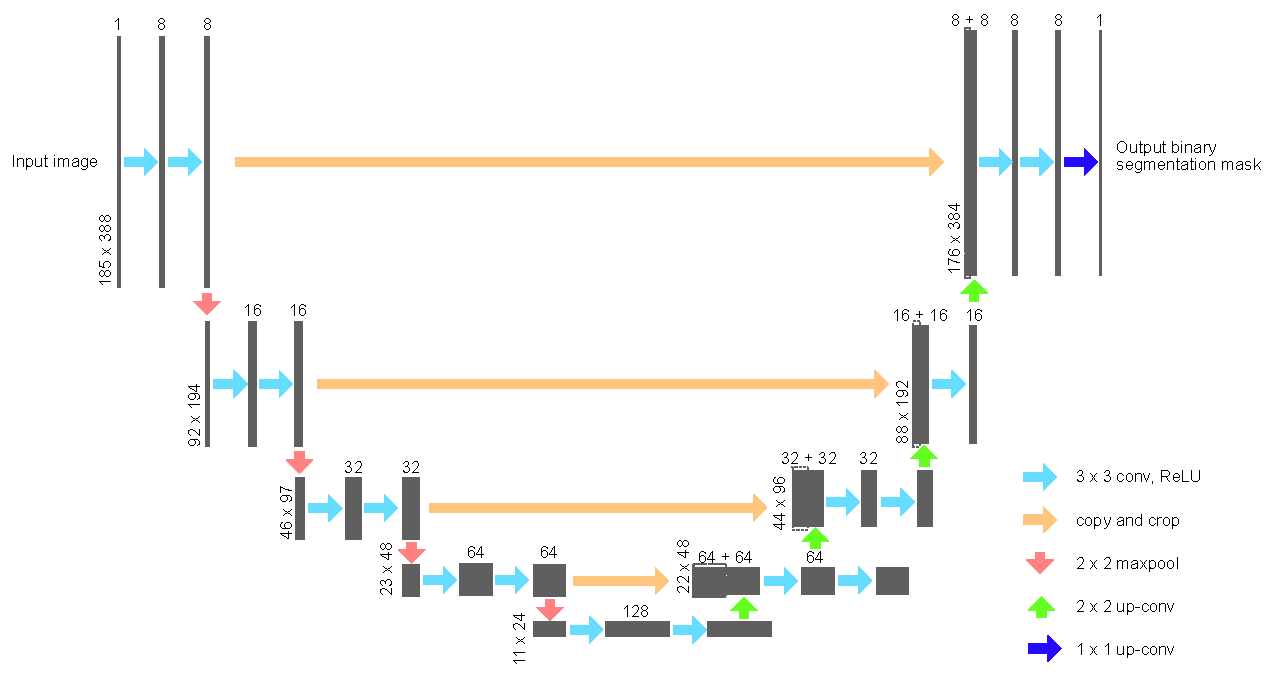
\includegraphics[width=0.9\textwidth,keepaspectratio]
{./figures/unet.pdf}
\caption{The U-Net architecture in \peaknet{}.}
\label{fig : unet}
\end{figure*}


\subsection{The loss function: focal loss}

A main technical issue in training U-Net for Bragg peak detection is the extreme
peak-background class imbalance (e.g., $> 10^3 : 1$), resulting in reduced
prediction accuracy.  This may not pose as a problem in previous peak finders
like BraggNet, which operates on a much smaller area of $32 \times 32$, whereas
\peaknet{} is trained on larger multi-panel detectors, such as the Cornell-SLAC
pixel array detector (CSPAD) \citep{hartCornellSLACPixelArray2012} with a
dimension of $194 \times 185$ for one of its panels.  Focal loss was introduced
to address the extreme class imbalance problem for object detectors
\citep{linFocalLossDense2018}.  It is defined as:

\begin{equation}
    \text{FL}(p) = -\alpha \cdot (1-p)^\gamma \cdot \log{p}.
\end{equation}

Here, $p$ is the probabilities of a pixel $x$ being a peak.  $\gamma$ controls a
modulating factor $(1-p)$ and $\alpha$ is an additional modulating factor.  We
used $\gamma = 2.0$ and $\alpha = 1.2$ in \peaknet{}.  In practice, numerical
instability will often emerge in the calculation of $p = e^{-\text{logit}}$,
where $\text{logit} = \log{(1 + e^{-x})}$.  To bypass this issue, logit needs to
be rewritten as $\text{logit} = a + \log{(e^{-a} + e^{-x-a})}$, where $a = max(0,
-x)$.  As a result, if we denote the label of a pixel $x$ as $y$, the focal loss
becomes

\begin{equation}
    \text{FL}(p) = \alpha \cdot y \cdot (1-p)^\gamma + \text{logit} + (1 - y)
    \cdot p^\gamma \cdot x + p^\gamma \cdot (1 - y) \cdot \text{logit}
\end{equation}


%%%%%%%%%%%%%%%%%%%%%%%%%%%%%%%%%%% DIVIDER %%%%%%%%%%%%%%%%%%%%%%%%%%%%%%%%%%%

\section{Experiments}

\subsection{\peaknet{} on multi-panel detectors: Trained on panels but
predicting on assembled images.}

We demonstrated the possibility of \peaknet{} making prediction on assembled
images from a multi-panel detector despite being trained on individual panels.
To facilitate this investigation, we utilized a multi-panel detector CSPAD,
which is widely used in serial crystallography experiments at LCLS.
Specifically, we used crystallographic data of streptavidin crystals from LCLS
experiment \textit{cxic0415} run \textit{101} at the Coherent X-ray Imaging (CXI)
instrument, where the CSPAD deployed consists of 32 panels.  An individual
diffraction image recorded on CSPAD are conventionally saved in a stack of 64
mini-panels (half of a physical CSPAD panel).  For data labeling, we randomly
selected 268 mini-panels, which were labeled using the \psocake{} peak finder
with the default settings.  We then split the labeled data into 60\% training
set and 20\% validation set.  The remaining 20\% data were initially set aside
for testing purposes, but were not used due to the lack of an effective metric,
which will be discussed later in the evaluation of our model's efficacy.  Our
test set included the first 5000 events of the run, which facilitated a faster
feedback loop compared with going through all events in the run.  Notably, we
did not apply any image preprocessing, and thus \peaknet{} directly takes in a
diffraction image of its original size and outputs a segmentation map.

\begin{figure*}[htbp]
\centering
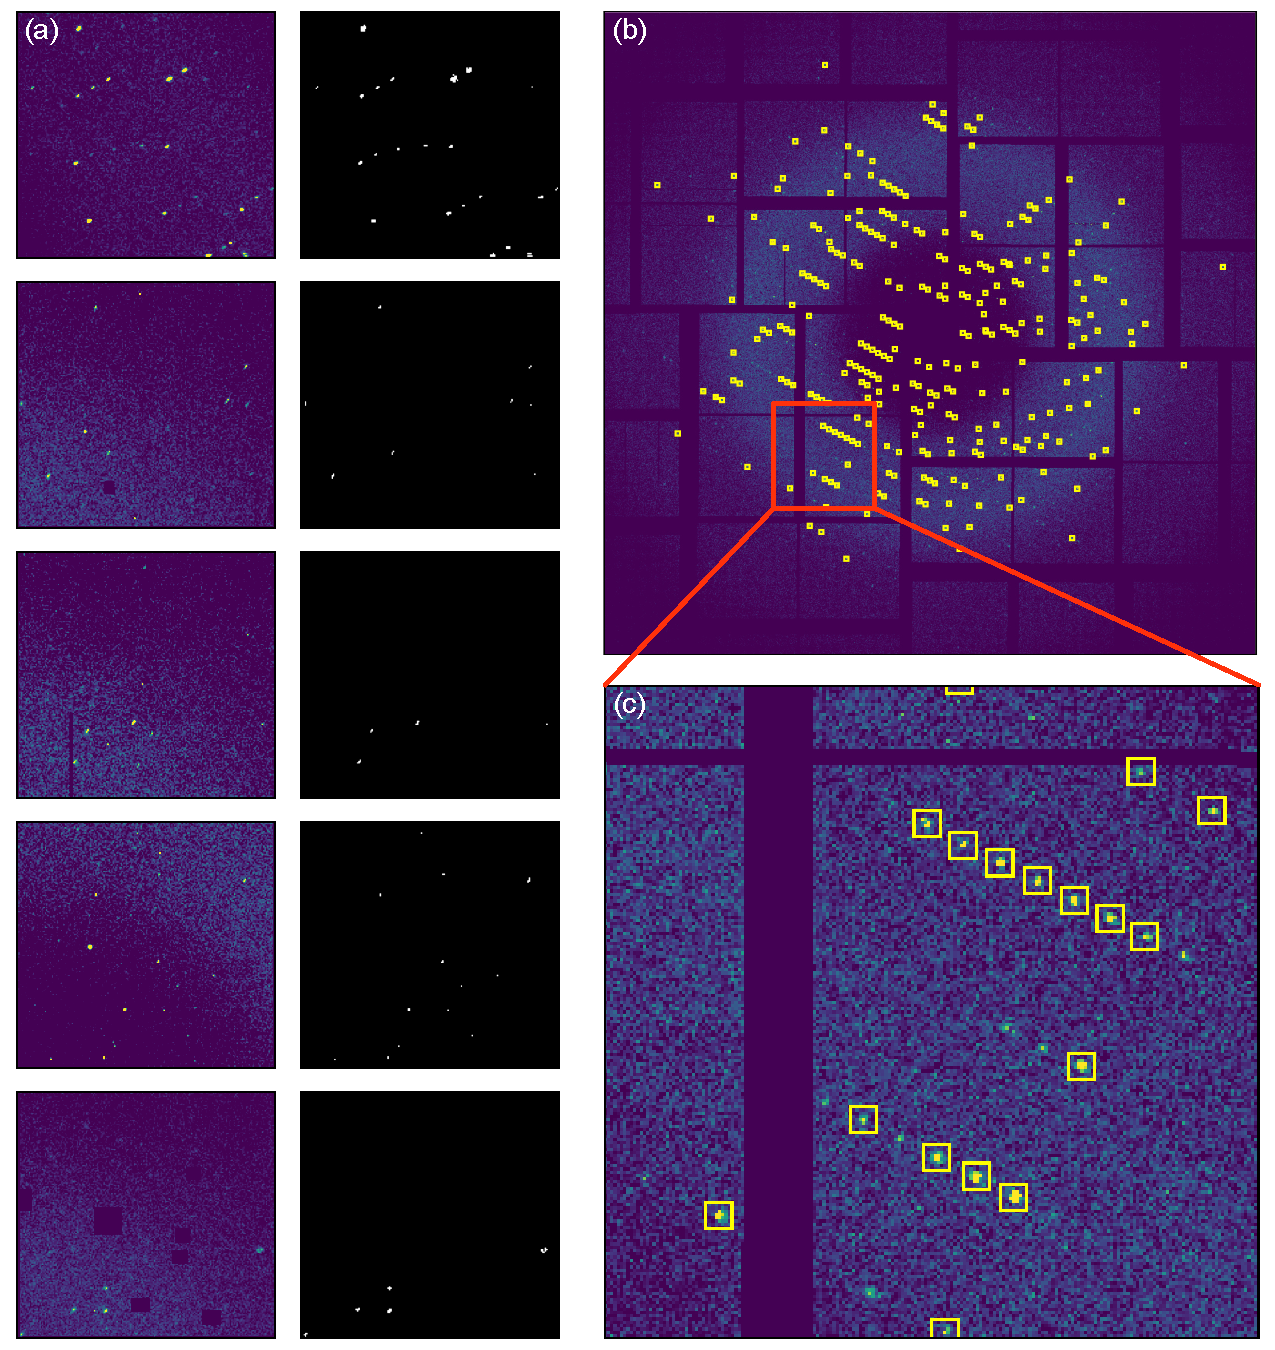
\includegraphics[width=0.9\textwidth,keepaspectratio]
{./figures/label_to_predict_with_zoom.pdf}
\caption{(a) \peaknet{} input images and peak labels.  (b) \peaknet{} prediction
on an entire CSPAD image.  (c) A magnified view of a small region of the
detector.}
\label{fig : label and predict}
\end{figure*}

Fig. \ref{fig : label and predict} (a) displays labeled samples, with the input
mini-panel image on the left and pixel-wise labeled peaks on the right.  The
overall peak label is a binary mask that shares the same size as the input, with
a value of one indicating a peak pixel and zero otherwise.  Consequently, each
input consists of a $185 \times 194$ mini-panel from the CSPAD and a binary mask
of the same size.  Additionally, Fig.  \ref{fig : label and predict} (b) shows a
sample model prediction on an entire CSPAD image with a size of $1739 \times
1748$.  


\subsection{Examining \peaknet{}'s generalizability beyound the peak finder used
in labeling}

The current strategy for data labeling involves using an existing peak finder,
and it is important to evaluate whether any limitations of the peak finder used
in data labeling will affect the peak finding capability of \peaknet{}. One
specific limitation to investigate is the size dependency of the peak finder.
Notably, the peak size range is a user-defined input requested by the \psocake{}
peak finder. This works well when diffraction spots have consistent sizes.
However, detectors such as the Rayonix have a large point spread function for
intense peaks, which may result in large peaks being ignored by the \psocake{}
peak finder.  Consequently, there is a concern about whether \peaknet{} will
inherit the same limitations since it is trained on \psocake{} peak labels.

\begin{figure*}[htbp]
\centering
\includegraphics[width=0.9\textwidth,keepaspectratio]
{./figures/rayonix.pdf}
\caption{Peak finding on a Rayonix image using (c) \peaknet{} and (d) \psocake{}.  (a), (b), (c) and (d) are magnified views of some regions.}
\label{fig : rayonix}
\end{figure*}

Fig. \ref{fig : rayonix} presents a side-by-side comparison of peak detection on
a Rayonix image, with the \peaknet{} results displayed on the left and the
\psocake{} results on the right.  The diffraction data were collected from
crystals of SARS-CoV-2 proteases using the Macromolecular Femtosecond
Crystallography (MFX) instrument
\citep{sierraMacromolecularFemtosecondCrystallography2019} at LCLS.  Upon visual
inspection of Fig. \ref{fig : rayonix} (c) and (d), both \peaknet{} and
\psocake{} were observed to detect a considerable number of peaks, suggesting a
potentially comparable performance between the two methods.  However, upon
closer inspection of the view near the area slightly below the beamstop position,
one obvious, reasonably sized Bragg peak was observed but not detected by the
\psocake{} peak finder, whereas \peaknet{} successfully located this peak.  This
finding provides direct evidence that \peaknet{}'s peak finding capability is
not strictly limited by the peak finder used in the data labeling process.  In
fact, \peaknet{} appears to possess its own understanding of Bragg peaks, as
evidenced by the exclusion of a weak single Bragg peak-like spot near the upper
edge of the image, as shown in Fig. \ref{fig : rayonix} (a) and (b).  Therefore,
it is important to note that \peaknet{} is not merely a neural network-based
replica of the \psocake{} peak finder despite being trained on labels supplied
by it.


\subsection{Model efficacy and runtime performance}

We consider model efficacy of a peak finder in two metrics: (1) indexing rate
and (2) the number of indexed events.  Table \ref{tb : perf} provides a
comparative analysis of two distinct datasets, CXI and MFX, showcasing the
outcomes obtained when processed using two peak finders, \psocake{} and
\peaknet{}.  The detectors employed for the respective datasets are CSPAD and
Rayonix.  The analyzed events for the CXI dataset span from 0 to 5000, whereas
the MFX dataset encompasses a range of 0 to 8998.  \psocake{} identified 2107
events in the CXI dataset and 465 in the MFX dataset, yielding indexing rates of
71.2\% and 84.5\%, respectively.  In contrast, \peaknet{} discovered 1991 events
in the CXI dataset and 430 in the MFX dataset, exhibiting superior indexing
rates of 78.6\% and 90.2\%, respectively.  Although both peak finders exhibit
varying levels of effectiveness, our evaluation has revealed that \peaknet{}
achieves superior indexing rates across both datasets, while also yielding
comparable numbers of indexed events.  These results suggest that \peaknet{} may
represent a more reliable and efficient solution for the analysis of such data.

To provide further context and justification for this efficacy measure, it is
important to note that conventional metrics like accuracy, precision and F-1
scores are not always well-defined in the context of peak finding, due to the
lack of actual ``ground truth".  This is because the peak labels used for
training and evaluation are derived from another peak finder, rather than being
uniquely determined in some fashion.  As a result, it is necessary to consider
alternative measures of model performance and reliability, such as the indexing
rate and the number of indexed events.  However, conventional metrics may remain
a viable option when applied to synthetic data generated by a simulator.   For
clarification purposes, we used the \textit{indexamajig} tool within the
\textit{CrystFEL} data analysis software \citep{whiteCrystFELSoftwareSuite2012}
to perform indexing.  We employed multiple indexing methods, including
\textit{mosflm}, \textit{xds} and \textit{xgandalf}, with an additional setting
of \textit{-int-radius=4,5,6}.   

\begin{table}[htbp]
\caption{
    Peak finding and indexing results.
}
\label{tb : perf}
\centering
\begin{tabular}{ | l || c | c | }
    \hline
    Dataset           &  CXI   & MFX\\
    \hline
    Detector          & CSPAD  & Rayonix \\
    Events to analyze & 0-5000 & 0-8998 \\
    \hline
    \psocake{}: Hits found         &  2107   & 465  \\
    \psocake{}: Indexed       &  1501   & 393  \\
    \psocake{}: Indexing rate &  71.2\% & 84.5\% \\
    \hline
    \peaknet{}: Hits found         &  1991   & 430  \\
    \peaknet{}: Indexed       &  1565   & 388  \\
    \peaknet{}: Indexing rate &  78.6\% & 90.2\% \\
    \hline
\end{tabular}
\end{table}

Furthermore, while the runtime performance of \peaknet{} is excellent as
compared with other crystallography data analysis methods in Table \ref{tb :
runtime}, there is a caveat to consider.  Although \peaknet{} is designed as a
nearly end-to-end solution, with its neural networks returning a segmentation
map that represents the pixel-wise probability of being a peak from input
diffraction images, we must employ connected component analysis to convert the
segmentation maps into peak coordinates.  While the neural network runtime is
exceptionally fast, capable of processing 11 Rayonix images ($1920 \times 1920$)
in parallel on a 1080 Ti GPU in just 4ms (equivalent to 0.36 ms per image), the
additional time required for connected component analysis is considerably longer
and thus a significant runtime bottleneck in the current version of \peaknet{}.
In fact, this bottleneck processing time scales nearly linearly with respect to
the number of images, and it adds an additional 30ms of processing time for each
image despite running on the same GPU.  Practically speaking, the current
version of \peaknet{} runs at 49ms per Rayonix event on 1080 Ti, which is
actually 10 $\times$ faster than some diffraction image classification
algorithms.


\begin{table*}[htbp]
\caption{
    The runtime performance of diffraction image analysis algorithms measured on
    Rayonix images containing 3.7 megapixels.  We measured runtime performance
    of \psocake{} and \peaknet{} directly using Rayonix images.  For reference
    purposes, we also included another peak finding method RPF
    \citep{hadian-jaziPeakfindingAlgorithmBased2017,
    hadian-jaziDataReductionSerial2021} and two classification methods for X-ray
    diffraction data reduction. RPF runtime performance was originally measured
    on AGIPD 1M \citep{allahgholiAdaptiveGainIntegrating2019}.  The two
    classification methods were evaluated on 0.5 megapixel images using the CNN
    hit finder method \citep{keConvolutionalNeuralNetworkbased2018}, which was
    also used as a point of comparison in the ORB+MLP method
    \citep{rahmaniDataReductionXray2023}. A $*$ notation was used to indicate a
    linearly extrapolated processing time, but the real performance may vary
    depending on the specific hardware and the complexity of the underlying
    algorithm.
}
\label{tb : runtime}
\centering
\begin{tabular}{  | l || l | l | c | c | }
    \hline
    Method      &  Task & Hardware & Image size           & Time (ms/event)  \\
    \hline
    RPF         &  Peak Finding & Intel E5-2698 & 1024 $\times$ 1024 & $\sim$120.0            \\
                &               &               & 1920 $\times$ 1920 &
                $\sim$421.8*            \\
    \hline
    \psocake{}  &  Peak Finding & Intel E5-2620 & 1920 $\times$ 1920 & 200.0             \\
    \hline
    \textbf{\peaknet{}}  &  Peak Finding & NVIDIA 1080 Ti & 1920 $\times$ 1920 &
    \textbf{49.0}            \\
    \hline
    CNN hit finder  & Classification & NVIDIA 1080 Ti &  720 $\times$ 720 & 0.8 \\
                                                     & &                & 1920
                                                      $\times$ 1920 & 5.6* \\
    \hline
    ORB+MLP  & Classification & Intel Core i5  & 720 $\times$ 720 & 50.0 \\
                                                     & &                & 1920
                                                      $\times$ 1920 & 355.6* \\
    \hline
\end{tabular}
\end{table*}


%%%%%%%%%%%%%%%%%%%%%%%%%%%%%%%%%%% DIVIDER %%%%%%%%%%%%%%%%%%%%%%%%%%%%%%%%%%%

\section{Conclusions}

In this paper, we introduced \peaknet{}, a deep learning-based peak finder that
efficiently tackles the Bragg peak finding problem as a semantic segmentation
task. The U-Net architecture of \peaknet{} has been optimized to achieve an
ideal balance between efficacy and runtime performance, resulting in a
processing speed four times faster than the \psocake{} peak finder while
maintaining superior indexing rates and a comparable number of indexed events. A
notable bottleneck in the current version of \peaknet{} is the connected
component analysis, which scales linearly with input data volume, whereas the
neural network portion scales beyond linear capability on GPUs, limited largely
by GPU memory. It is worth mentioning that the current data reduction concept
primarily focuses on processing single events as quickly as possible, centering
the design principle on CPUs. However, with neural networks, we propose a new
direction towards batch image processing on GPUs, exemplified by \peaknet{} in
the context of serial crystallography.

%%%%%%%%%%%%%%%%%%%%%%%%%%%%%%%%%%% DIVIDER %%%%%%%%%%%%%%%%%%%%%%%%%%%%%%%%%%%

\section*{Acknowledgment}

Earlier versions of the U-Net models were built and tested by P.L under the
supervision of C.H.Y.  The experiments were designed by C.W with inputs from
J.B.T and C.H.Y.  C.W prepared the datasets, labeled experimental data, and
trained and evaluated the refined neural network model.  The manuscript was
written by C.W and C.H.Y with input from all authors.  This material is based
upon work supported by the U.S.  Department of Energy, Office of Science, Office
of Basic Energy Sciences under Award Number FWP-100643.  Use of the Linac
Coherent Light Source (LCLS), SLAC National Accelerator Laboratory, is supported
by the U.S. Department of Energy, Office of Science, Office of Basic Energy
Sciences under Contract No.  DE-AC02-76SF00515.

\bibliographystyle{plainnat}
\bibliography{bibliography.bib}

\end{document}

